\section{Model generalizations} \label{sec:model2}

\subsection{Poisson observations}
\paragraph{Model}

\begin{align}
	F_t \sim \text{Poisson}(\alpha (C_t + \beta))
\end{align}

% \begin{align}
% 	\bF_{x,t} \sim \text{Poisson}(\alpha_x (C_t + \beta))
% \end{align}

\paragraph{Inference}

\begin{subequations} 
\begin{align}
\mL_{t} &= \alpha (C_t + \beta) - F_{t} \log(\alpha(C_t + \beta)) + \log(F_{t}!)  \\
g_{t} &= \alpha - F_{t}(C_t + \beta)^{-1} \\
H_{t} &= F_{t} (C_t + \beta)^{-2}
\end{align}
\end{subequations}

\noindent where $\mL=\sum_{t} \mL_{t}$, $\bg=(g_{1}, \ldots, g_{T})\T$, and $\bH=\text{diag}((H_1, \ldots, H_T))$.

\begin{figure}[h!]
\centering 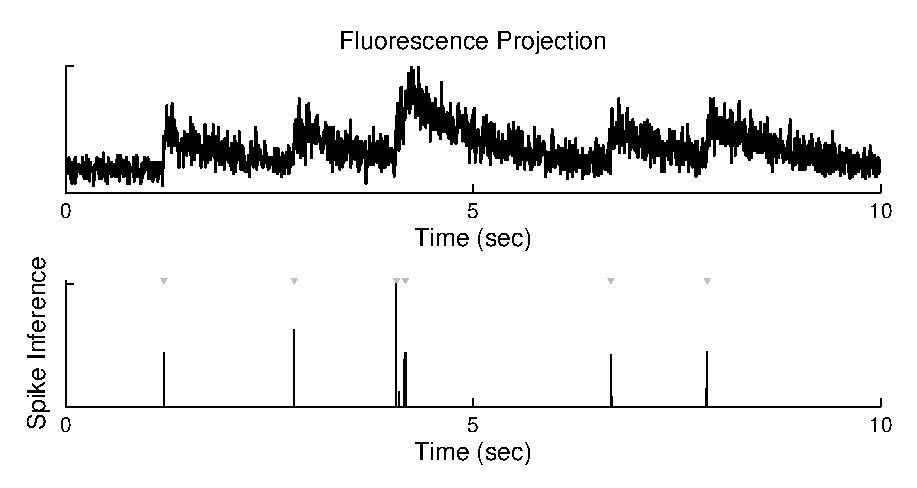
\includegraphics[width=.9\linewidth]{../figs/poisson}
\caption{Poisson} \label{fig:poiss}
\end{figure}


\subsection{Nonlinear observations}
\paragraph{Model}

\begin{align}
	F_t = \alpha \frac{C_t}{C_t + k_d} + \beta + \sig \varepsilon_t
\end{align}

\paragraph{Inference}

\begin{subequations} 
\begin{align}
\mL &= \frac{1}{2\sig^2} \norm{\bF - \alpha\left( \frac{\bC}{\bC+k_d} + \beta\right)}^2 + (\bM \bC)\T \blam - z \log (\bM\bC)\T \ve{1}  \\
g &= -2 \alpha k_d (\bF - \bC - \beta)\T  \ast (C+k_d)^{-2} + \bM\T\blam - z \bM\T (\bM\bC)^{-1} \\
H_{t} &= -\alpha k_d - 2(\bC + k_d) \ast (\bF-\bC-\beta) \ast (\bC + k_d)^{-4} + z \bM\T (\bM \bC)^{-2} \bM
\end{align}
\end{subequations}

\noindent where $\ast$ indicates an element-wise multiplication and the exponents are all taken element-wise as well. Because the Hessian is not positive-semi-definite, this optimization problem is not concave.  Therefore, we provide an initial condition by first using the linear observation model.  

\begin{figure}[h!]
\centering 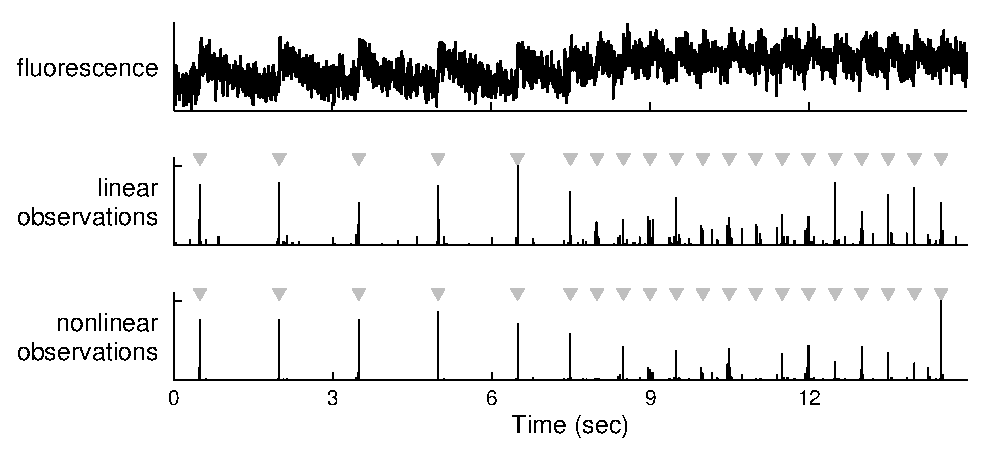
\includegraphics[width=.9\linewidth]{../figs/nonlin}
\caption{Saturation} \label{fig:satur}
\end{figure}

\subsection{Slow rise time}

\subsection{External stimulus}

\paragraph{Model}


\begin{align}
	n_t &\sim \text{Poisson}(n_t; \lam_t \Del)
\end{align}

\paragraph{Inference}

Above, we defined $\blam=\lam\Del\ve{1}\T$.  Here, $\blam=(\lam_1, \ldots, \lam_T) \Del$.  Everything follows as before.

\begin{figure}[h!]
\centering 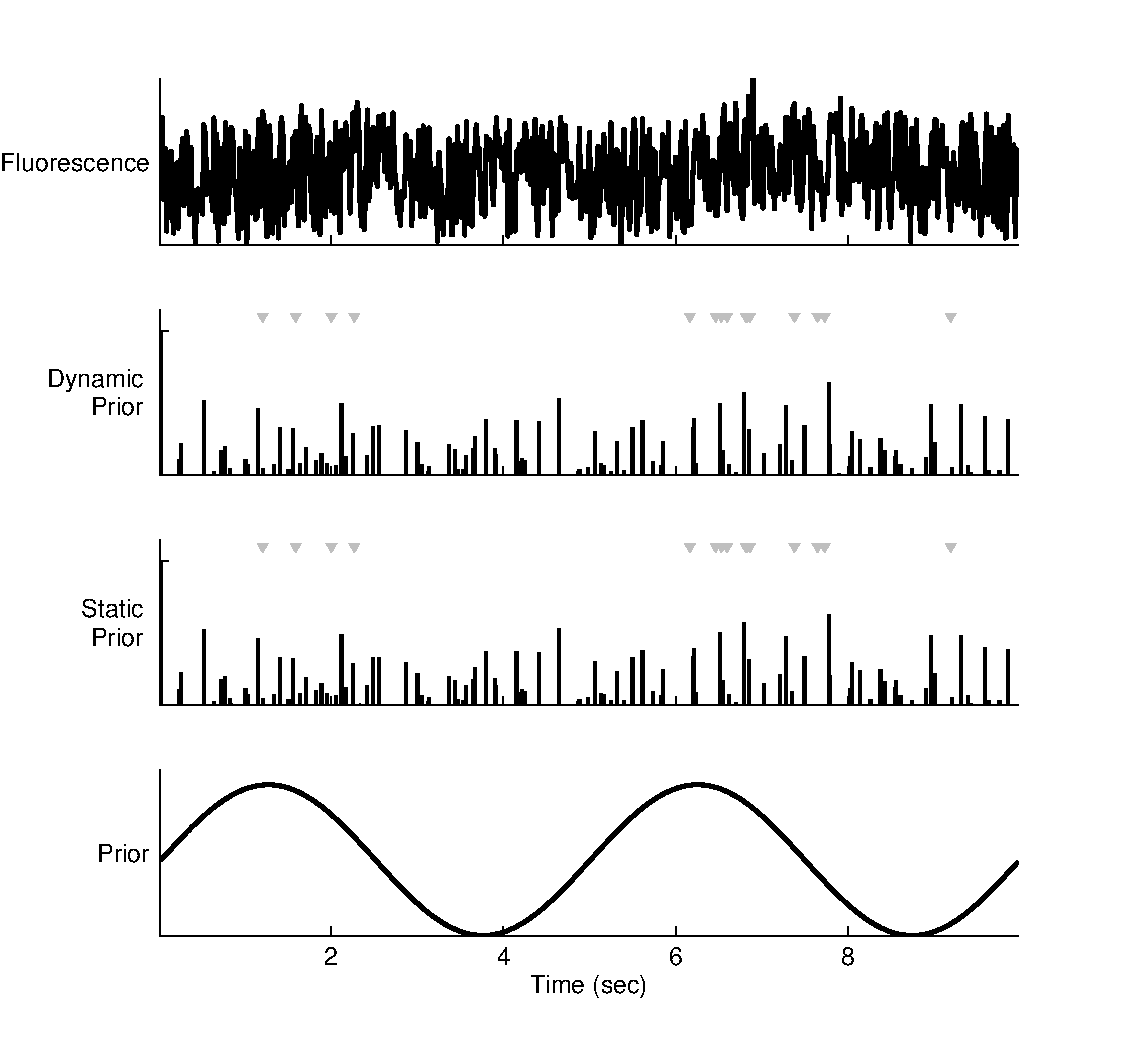
\includegraphics[width=.9\linewidth]{../figs/dynamic_prior}
\caption{Can't find a regime in which it helps.} \label{fig:woopsi}
\end{figure}


